\documentclass[a4paper, 12pt, openany]{book}

%%% Работа с русским языком % для pdfLatex
\usepackage{cmap}					% поиск в~PDF
\usepackage{mathtext} 				% русские буквы в~фомулах
\usepackage[T2A]{fontenc}			% кодировка
\usepackage[utf8]{inputenc}			% кодировка исходного текста
\usepackage[english,russian]{babel}	% локализация и переносы
\usepackage{indentfirst} 			% отступ 1 абзаца
\usepackage{gensymb}				% мат символы?

%%% Работа с русским языком % для XeLatex
%\usepackage[english,russian]{babel}   %% загружает пакет многоязыковой вёрстки
%\usepackage{fontspec}      %% подготавливает загрузку шрифтов Open Type, True Type и др.
%\defaultfontfeatures{Ligatures={TeX},Renderer=Basic}  %% свойства шрифтов по умолчанию
%\setmainfont[Ligatures={TeX,Historic}]{Times New Roman} %% задаёт основной шрифт документа
%\setsansfont{Comic Sans MS}                    %% задаёт шрифт без засечек
%\setmonofont{Courier New}
%\usepackage{indentfirst}
%\frenchspacing

%%% Дополнительная работа с математикой
\usepackage{amsfonts,amssymb,amsthm,mathtools}
\usepackage{amsmath}
\usepackage{icomma} % "Умная" запятая: $0,2$ --- число, $0, 2$ --- перечисление
\usepackage{upgreek}

%% Номера формул
%\mathtoolsset{showonlyrefs=true} % Показывать номера только у тех формул, на которые есть \eqref{} в~тексте.

%%% Страница
\usepackage{extsizes} % Возможность сделать 14-й шрифт

%% Шрифты
\usepackage{euscript}	 % Шрифт Евклид
\usepackage{mathrsfs} % Красивый матшрифт

%% Свои команды
\DeclareMathOperator{\sgn}{\mathop{sgn}} % создание новой конанды \sgn (типо как \sin)
\DeclareMathOperator{\rg}{\mathop{rg}}
\DeclareMathOperator{\Rg}{\mathop{Rg}}
\DeclareMathOperator{\im}{\mathop{Im}}
\DeclareMathOperator{\tr}{\mathop{tr}}
\DeclareMathOperator{\const}{\mathop{const}}
\DeclareMathOperator{\Id}{\mathop{Id}}
%\DeclareMathOperator{\dim}{\mathop{dim}}
\usepackage{csquotes} % ещё одна штука для цитат
\newcommand{\pd}[2]{\ensuremath{\cfrac{\partial #1}{\partial #2}}} % частная производная
\newcommand{\abs}[1]{\ensuremath{\left|#1\right|}} % модуль
\renewcommand{\phi}{\ensuremath{\varphi}} % греческая фи
\newcommand{\pogk}[1]{\!\left(\cfrac{\sigma_{#1}}{#1}\right)^{\!\!\!2}\!} % для погрешностей


%\renewcommand{\labelenumi}{\asbuk{enumi})}

% Ссылки
\usepackage{color} % подключить пакет color
% выбрать цвета
\definecolor{BlueGreen}{RGB}{49,152,255}
\definecolor{Violet}{RGB}{120,80,120}
% назначить цвета при подключении hyperref
\usepackage[unicode, colorlinks, urlcolor=blue, linkcolor=blue, pagecolor=blue, citecolor=blue]{hyperref} %синие ссылки
%\usepackage[unicode, colorlinks, urlcolor=black, linkcolor=black, pagecolor=black, citecolor=black]{hyperref} % для печати (отключить верхний!)


%% Перенос знаков в~формулах (по Львовскому)
\newcommand*{\hm}[1]{#1\nobreak\discretionary{}
	{\hbox{$\mathsurround=0pt #1$}}{}}

%%% Работа с картинками
\usepackage{graphicx}  % Для вставки рисунков
\graphicspath{{images/}{images2/}}  % папки с картинками
\setlength\fboxsep{3pt} % Отступ рамки \fbox{} от рисунка
\setlength\fboxrule{1pt} % Толщина линий рамки \fbox{}
\usepackage{wrapfig} % Обтекание рисунков и таблиц текстом
\usepackage{multicol}

%%% Работа с таблицами
\usepackage{array,tabularx,tabulary,booktabs} % Дополнительная работа с таблицами
\usepackage{longtable}  % Длинные таблицы
\usepackage{multirow} % Слияние строк в~таблице
\usepackage{caption}
\captionsetup{labelsep=period, labelfont=bf}

%%% Оформление
\usepackage{indentfirst} % Красная строка
%\setlength{\parskip}{0.3cm} % отступы между абзацами
%%% Название разделов
\usepackage{titlesec}
\titlelabel{\thetitle.\quad}
\renewcommand{\figurename}{\textbf{Рис.}}		%Чтобы вместо figure под рисунками писал "рис"
\renewcommand{\tablename}{\textbf{Таблица}}		%Чтобы вместо table над таблицами писал Таблица
\usepackage{enumitem}
\setlist{nolistsep}
\usepackage{verbatim}

%%% Теоремы
\theoremstyle{plain} % Это стиль по умолчанию, его можно не переопределять.
\newtheorem{theorem}{Теорема}[section]
\newtheorem{proposition}[theorem]{Утверждение}
\newtheorem{predlog}{Предложение}[section]
\newtheorem{lemma}{Лемма}[section]

\theoremstyle{definition} % "Определение"
\newtheorem{definition}{Определение}[section]
\newtheorem{corollary}{Следствие}[theorem]
\newtheorem{problem}{Задача}[section]

\theoremstyle{remark} % "Примечание"
\newtheorem*{nonum}{Решение}
\newtheorem{zamech}{Замечание}[theorem]

%%% Правильные мат. символы для русского языка
\renewcommand{\epsilon}{\ensuremath{\varepsilon}}
\renewcommand{\phi}{\ensuremath{\varphi}}
\renewcommand{\kappa}{\ensuremath{\varkappa}}
\renewcommand{\le}{\ensuremath{\leqslant}}
\renewcommand{\leq}{\ensuremath{\leqslant}}
\renewcommand{\ge}{\ensuremath{\geqslant}}
\renewcommand{\geq}{\ensuremath{\geqslant}}
\renewcommand{\emptyset}{\varnothing}

%%% Для лекций по инфе
\usepackage{alltt}
\newcounter{infa}[section]
\newcounter{num}
\definecolor{infa}{rgb}{0, 0.2, 0.89}
\definecolor{infa1}{rgb}{0, 0.3, 1}
\definecolor{grey}{rgb}{0.5, 0.5, 0.5}
\newcommand{\tab}{\ \ \ }
\newcommand{\com}[1]{{\color{grey}\##1}}
\newcommand{\num}{\addtocounter{num}{1}\arabic{num}\tab}
\newcommand{\defi}{{\color{infa}def}}
\newcommand{\ini}{{\color{infa}in}}
\newcommand{\rangei}{{\color{infa}range}}
\newcommand{\fori}{{\color{infa}for}}
\newcommand{\ifi}{{\color{infa}if}}
\newcommand{\elsei}{{\color{infa}else}}
\newcommand{\printi}{{\color{infa1}print}}
\newcommand{\maxi}{{\color{infa}max}}
\newcommand{\classi}{{\color{infa}class}}
\newcommand{\returni}{{\color{infa}return}}
\newcommand{\elifi}{{\color{infa}elif}}


\newenvironment{infa}[1]{
	
	\vspace{0.5cm}
	\addtocounter{infa}{1}%
	\noindent{\large \textbf{Программа №\thesection.\arabic{infa}}}\textbf{<<#1>>}%
	\begin{alltt}%
	}{\end{alltt}
	\setcounter{num}{0}
	\vspace{0.1cm}}
%Пример кода:
%\begin{infa}{Поразрядная сортировка}
%	\ \num \defi count_sort(a):\tab \com{определяет нашу функцию}
%	\ \num \tab m = \maxi(a)+1
%	\ \num \tab q = [0]*m
%	\ \num \tab \fori x \ini a:
%	\ \num \tab \tab q[x] += 1
%	\ \num \tab pos = 0
%	\ \num \tab \fori x \ini q:
%	\ \num \tab \tab \fori i \ini \rangei(q[x]):
%	\ \num \tab \tab \tab a[pos] = x
%	\num \tab \tab \tab pos += 1
%\end{infa}

\usepackage{titlesec}
\titlelabel{\thetitle.\quad}

\title{Вопрос по выбору}
\author{Алексей Кожарин}
\date{\today}
\usepackage[left=1.27cm,right=1.27cm,top=2cm,bottom=2cm]{geometry}

\usepackage{fancyhdr} % Для колонтитулов

\renewcommand{\baselinestretch}{1.3}

\makeatletter % Убирает нумерацию на страницах, где \chapter
\renewcommand\chapter{\if@openright\cleardoublepage\else\clearpage\fi
	\thispagestyle{empty}% original style: plain
	\global\@topnum\z@
	\@afterindentfalse
	\secdef\@chapter\@schapter}
\makeatother

\usepackage{fancyhdr}
\pagestyle{fancy}
\fancyhf{}
\fancyhead[L]{\rightmark}
\fancyhead[R]{\textbf{\thepage}}

\setcounter{secnumdepth}{0}

\newcommand\invisiblesection[1]{%
	\refstepcounter{section}%
	\addcontentsline{toc}{section}{#1}%
	\sectionmark{#1}}


\begin{document}
	\begin{titlepage}
\begin{center} 
 
\large Московский физико-технический институт\\
Физтех-школа электроники фотоники и молекулярной физики\\
\vspace{6cm}
\huge Вопрос по выбору \\\ \\ Использование спектрографии в исследовании небесных объектов
\end{center} 

\vspace{7cm}
{\par \raggedleft \large \emph{Выполнил:}\\ студент 2 курса\\ Б04-005 группы ФЭФМ\\ Давыдов Владислав\\ Олегович \par}
\begin{center}
\vfill Москва \today
\end{center}
\end{titlepage}
\newpage
\setcounter{page}{2}
	
	\invisiblesection{Использование спектрографии в исследовании небесных объектов}
	\section{Предисловие}
	\textbf{SN 2009ip} сверхновая вспыхнула в сентябре 2012 года после нескольких предварительных вспышек. Сверхновая располагалась в галактике NGC 7259. В контексте данной задачи мы попытаемся оценить угловой диаметр туманности появившийся из остатков сверхновой на момент июня 2022 года. Также, будем пренебрегать вкладом предварительных вспышек в формирование газопылевого облака.
		
	\section{Обработка данных}
	\begin{wrapfigure}{l}{0.56\textwidth}

		\center{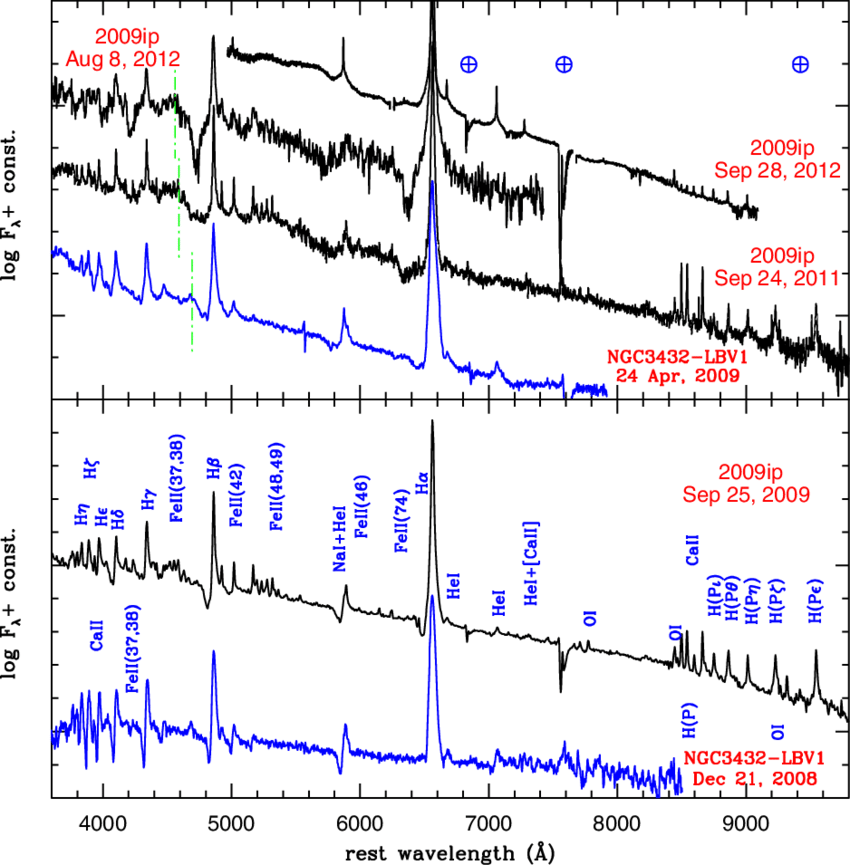
\includegraphics[width=\linewidth]{spectra}}
		\caption{ Спектр сверхновой SN 2009ip \\
			Мы будем использовать спектр водорода.
		}
		\label{pic1}
	\end{wrapfigure}
	Из открытых источников определим расстояние до галактики в которой происходит коллапс. Примем его равным $L = 25 $ Мпк (1пк = 206265 а.е). Далее, мы будем рассматривать спектры сверхновой. В них присутствуют яркие эмиссионные линии атомарного водорода, самая заметная из которых - $H \alpha$ с длиной волны около 6560 ангстрем. Однако левее этой линии, на чуть меньших длинах волн, видна достаточно четкая линия поглощения. Это не есть случайная близость двух линий - такая же компонента присутствует и у линии $H \beta$ . Эта линия - результат поглощения света быстро расширяющейся оболочкой взорвавшейся звезды. Ее разные участки имеют разные направления скорости, но с Земли сильнее всего проявляет себя часть оболочки, летящая по направлению к нам. За счет очень большой скорости линия поглощения смещена в фиолетовую сторону относительно линии излучения самой звезды. Именно эту скорость мы будем определять из спектра.	
	
	\newpage
	
	Необходимо учитывать, что разные молекулы газа имеют разные скорости, что приводит к значительной ширине линии поглощения. Так как нас интересуют размеры туманности или, строго говоря, угловое расстояние до ее видимого центра до края, мы будем рассматривать самые быстрые молекулы, создающие левый край спектральной линии. Из графика определим длину волны левого крыла линии поглощения и линии излучения $H \alpha $ самой звезды:
	\begin{equation}
	\label{eq1}
	\lambda = 6000A + \dfrac{51}{127} * 1000A = 6402 A
	\end{equation}
	\begin{equation}
	\label{eq2}
	\lambda_{0} = 6000 A + \dfrac{72}{127} *1000A = 6567 A
	\end{equation}
	
	Длина волны $\lambda_{0}$ близка к лабораторной длине волны $H \alpha$ , однако на нее, вообще гворя может влиять лучевая скорость самой сверхновой звезды и ее галактики в целом. Отсюда получаем лучевую скорость самых быстрых атомов:
	
	\begin{equation}
	\label{eq3}
	\upsilon_{\alpha} = c \dfrac{\lambda_{0} - \lambda}{\lambda_{0}} =  7500 \; km/s
	\end{equation}
	
	Попробуем определить по линии $H \beta$ :
	4882  4780
	\begin{equation}
	\label{eq4}
	\lambda_{b} = 4780 A
	\end{equation}
	\begin{equation}
	\label{eq5}
	\lambda_{b0} = 4882 A
	\end{equation}
	
	\begin{equation}
	\label{eq6}
	\upsilon_{\beta} = c \dfrac{\lambda_{b0} - \lambda_{b}}{\lambda_{b0}} =  6300 \; km/s
	\end{equation}
	
	
	За оценку лучевой скорости будем брать $\upsilon = 7000 \; km/s $

	\section{Теоретическая модель}
	
Полученная скорость очень велика, несопоставимо выше второй космической для окрестностей звезды,  но все же заметно меньше скорости света. Поэтому для определения углового диаметра для наблюдения в 2022 году достаточно определить ее линейный диаметр через время $T = 9.75$ лет после взрыва и поделить на расстояние:
	\begin{equation}
	\label{eq7}
	\rho = \dfrac{2 \upsilon T}{L} = \dfrac{4.3*10^{12} km}{7.7 * 10^{17} km} = 6 * 10^{-6} = 1''.
	\end{equation}
	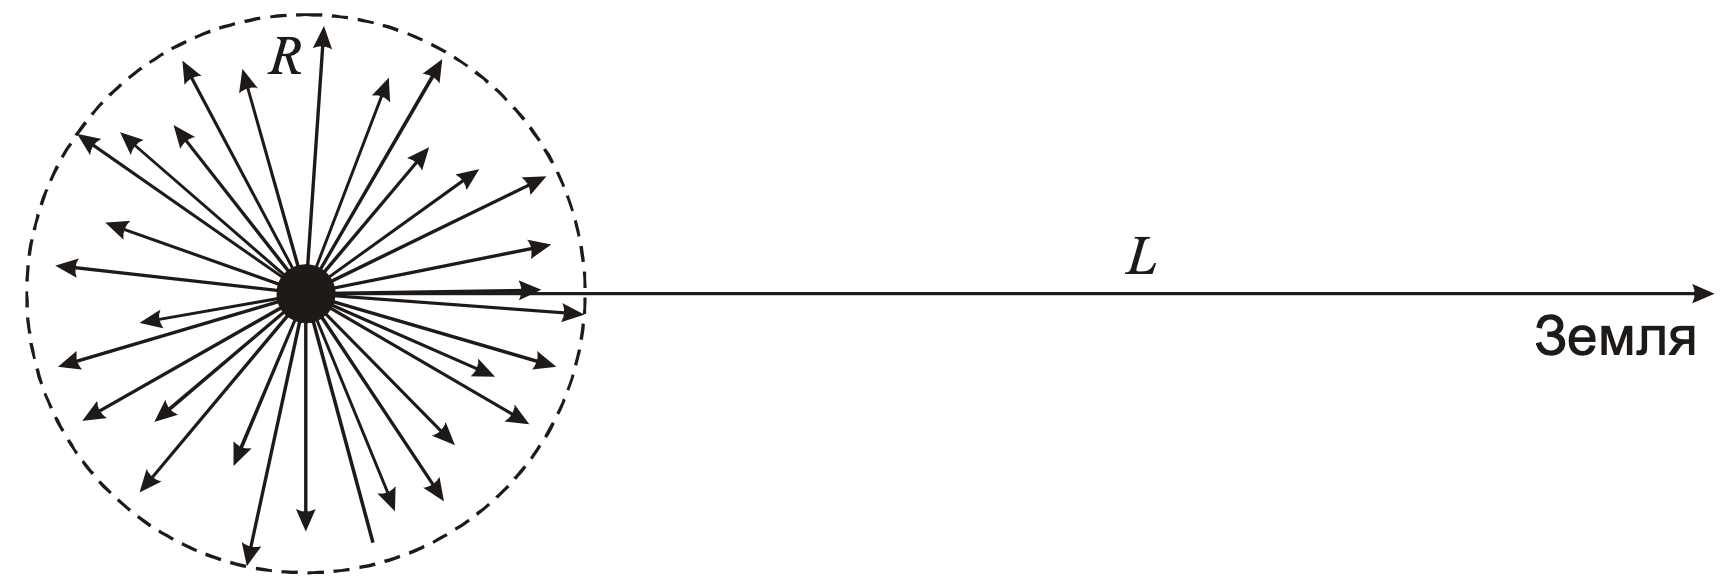
\includegraphics[scale=0.6]{shema}  
	
	\newpage
	\begin{centering}
	\section{Литература}
	\begin{itemize}
	\item Ландсберг Г.С. , "Оптика" , 2010, 978-5-9221-0314-5
	\item Andrea Pastorello and Cosimo Inserra, "Interacting Supernovae and Supernova Impostors. SN 2009ip, is this the end?", October 2012, The Astrophysical Journal 767(1), 10.1088/0004-637X/767/1/1
	\item Угольников О.С, XXV Всероссийская олимпиада школьников по астрономии, Волгоград 2018
	\end{itemize}
	\end{centering}

\end{document}